  \subsection{Dépendances et Relations}
  Le programme est simple d'utilisation puisqu'il suffit de le lancer
  avec un fichier d'entrée de type graphe issu du programme
  \emph{gengraph} de
  \emph{C. Gavoille}\footnote{\url{http://dept-info.labri.fr/~gavoille/gengraph.c}}
  ainsi qu'avec le numéro du problème et éventuellement des paramètres
  propres au problème.\\
  Le programme se déroule de la manière suivante :
  \begin{enumerate}
   \item Le fichier de graphe est lu à partir du fichier de graphe
	 fourni. 
   \item Selon le problème sélectionné, on lance la réduction
	 correspondante. 
   \item Une formulation en clauses de type \emph{CNF} est créée et
	 envoyée au \emph{SATSolver} \emph{Minisat}. 
   \item \emph{Minisat} crée une solution (si cela est possible).
   \item La solution fournie est analysée afin de pouvoir être
	 traitée. De cette manière, nous connaissons la solution au
	 problème voulu sur le graphe passé en paramètre. 
  \end{enumerate}
  
  En décrivant l'exécution du programme de cette façon, il est aisé de
  voir apparaître les relations entre les modules de notre programme.

  La fonction principale \emph{main}, contenue dans \emph{Solve.cpp},
  joue le rôle du tri des arguments et de construction du
  graphe. Ensuite, est appelée la réduction voulue, contenue dans les
  fichiers portant le nom d'un problème (ou leur abréviation). Une fois
  la réduction effectuée par ce fichier, celui-ci appelle un ``parser''
  pour \emph{Minisat} (dans \emph{MinisatBuilder.cpp}) qui gère le fait
  d'écrire un fichier d'entrée à \emph{Minisat}, de lancer le
  \emph{SAT-Solver} et d'analyser sa sortie. Une fois la sortie
  analysée, une assignation des variables est donnée. Celle-ci nous
  permet alors de fournir l'ensemble des arêtes ou sommets nécessaire
  définissant une solution du problème donné sur le graphe donné.\\

  Voici un graphe représentant simplement les relations entre les
  différentes parties du programme (fig.\ref{grapheExec} page
  \pageref{grapheExec}).
  \begin{figure}[!ht]
   \begin{center}
    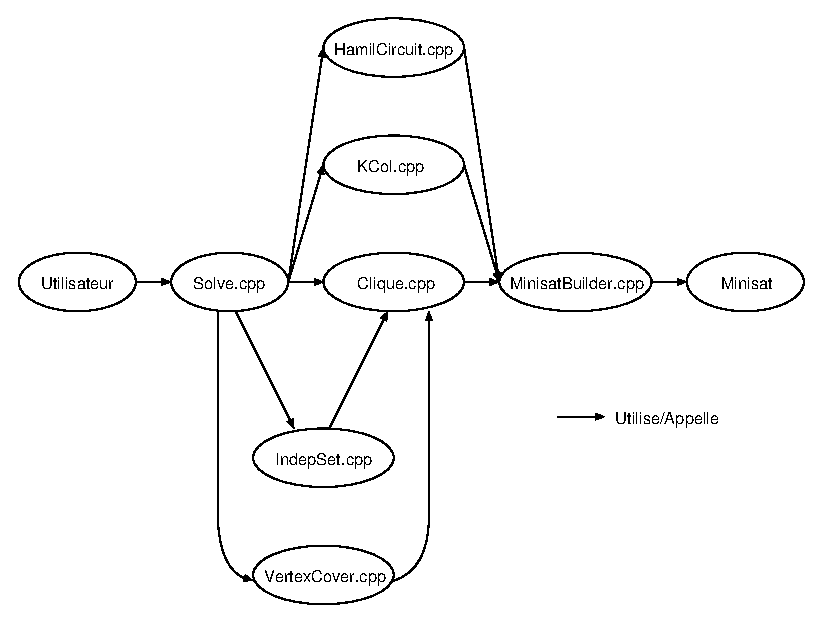
\includegraphics{images/grapheExec.eps}
    \caption{Relations entre les différentes parties du
    programme\label{grapheExec}}
   \end{center}
  \end{figure}